\begin{frame}
    \begin{itemize}
        \item The block chain provides Bitcoin's public ledger, an ordered and timestamped record of transctions.
        \item This system is used to protect against double spending and modification of previous transactions records.
        \item Each full node in the Bitcoin network independently stores a block chain containing only blocks validated by that node.
    \end{itemize}
\end{frame}

\begin{frame}
    \frametitle{Block Chian Overview}
    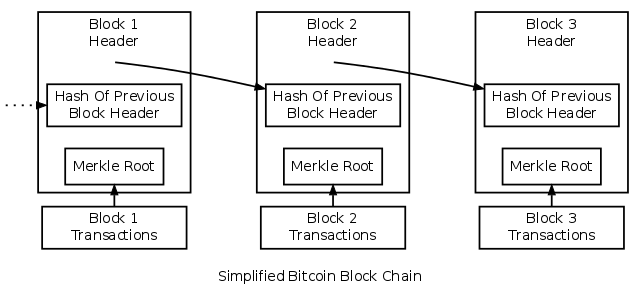
\includegraphics[scale=0.4]{./figures/en-blockchain-overview.png}
\end{frame}

\begin{frame}
    \frametitle{Hard Fork}
    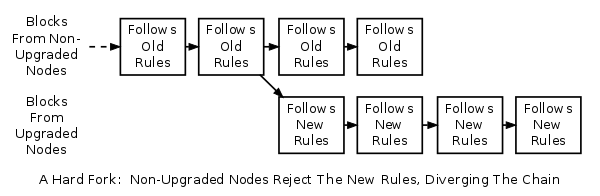
\includegraphics[scale=0.4]{./figures/en-hard-fork.png}
\end{frame}

\begin{frame}
    \frametitle{Soft Fork}
    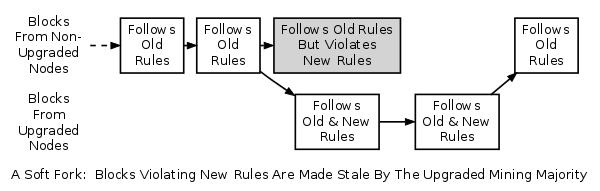
\includegraphics[scale=0.4]{./figures/en-soft-fork.png}
\end{frame}
